\documentclass[tikz, border=3mm]{standalone}
\usepackage{tikz}
\usetikzlibrary{arrows.meta}

\begin{document}
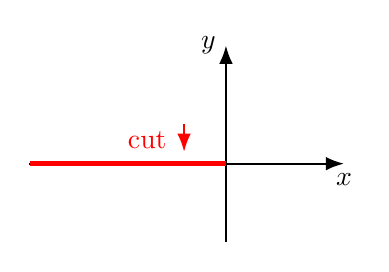
\begin{tikzpicture}[
    >=Latex % Set default arrow tip style
]

    % Axes
    \draw[->, thick] (-2.5, 0) -- (1.5, 0) node[below] {$x$}; % x-axis
    \draw[->, thick] (0, -1) -- (0, 1.5) node[left] {$y$}; % y-axis

    % Red Cut Line along negative x-axis
    \draw[red, ultra thick] (-2.49, 0) -- (0, 0);

    % Label "cut" above the line
    \node[red] (cutlabel) at (-1, 0.3) {cut};

    % Small downward arrow near the label
    \draw[->, red, thick] (cutlabel.east) ++(0.1, 00.2) -- ++(0, -0.35); % Start right of label, draw down

\end{tikzpicture}
\end{document}